\documentclass[
    8.2pt,
    a4paper,
    logo,
    twocolumn
]{template}


\usepackage[most]{tcolorbox}
\usepackage{mathtools, cuted}
\usepackage{hyperref}              % hyperlinks
\usepackage{url}                   % simple URL typesetting
\usepackage{booktabs}              % professional-quality tables
\usepackage{amsfonts}              % blackboard math symbols
% \usepackage{amsthm}                % Theorem environments.
\usepackage{nicefrac}              % compact symbols for 1/2, etc.
\usepackage{microtype}             % microtypography
\usepackage{xcolor}                % colored text
\usepackage{graphicx}              % graphics
\usepackage{amsmath}               % AMS math package
\usepackage{amssymb}               % AMS symbols
\usepackage{wrapfig}               % Wrap figures
\usepackage{lipsum}                % Lorem Ipsum
\usepackage{booktabs}              % Beautiful tables
\usepackage{appendix}
\usepackage{enumerate}
\usepackage[sort&compress]{natbib}
\bibliographystyle{abbrvnat}

%%%%%%%% CUSTOM
\newtheorem{lemma}{Lemme}
\newtheorem{theorem}{Théorème}
\newtheorem{corollary}{Corollaire}
\newtheorem{definition}{Définition}
\newtheorem{remarque}{Remarques}
\newtheorem{proposition}{Proposition}

% Resize / Scale equations
\newcommand\scalemath[2]{\scalebox{#1}{\mbox{\ensuremath{\displaystyle #2}}}}

\renewcommand{\min}{\inf}

%%%%%%%% CONTENT
\title{Introduction à la théorie du transport optimal}

% Use the internally issued paper ID, if there is one
\reportnumber{001} % Leave blank if n/a

% Assign your own date to the report.
% Can comment out if not needed or leave blank if n/a.
\renewcommand{\today}{12 Janvier 2022}

% Can have as many authors and as many affiliations as needed. Best to indicate joint
% first-authorship as shown below.
% \author[*]{}
\author[*]{Aymen Lakhyar}
\author[*]{Badr-Eddine Marani}
\author[*]{Mohamed Amine Hasnabi}
\author[*]{Othmane Mirinioui}
\author[*]{Oumaima Et-Tahri}
\author[*]{Oussama Mouhtal}

% Affiliations *must* come after the declaration of \author[]
\affil[*]{Ecole Centrale Casablanca}

\begin{abstract}
    \paragraph{\textit{Abstract.}} In this paper, we introduce the theory of optimal transport as it was formulated by Gaspard Monge and Kantorovitch and its formulation in a more general context by measure and probability theories.  We discuss some mathematical aspects of this problem in order to introduce the notion of duality and the theorems of existence and characterization of optimal transports.

    Therefore, We show how optimal transport theory can be used for a wide range of practical problems, by showing how Optimal Transport problem can allow us to define the Wasserstein distance, which captures the most natural geometry in the space of probability measures. Finally, we present  one of these practical problems (MRI (Magnetic Resonance Imagery) paper, also matching and pricing in two-side market.
\end{abstract}

\begin{document}
    \maketitle
    \section{La théorie du transport optimal}
    \subsection{Formulation de Monge}\label{sec:introduction}
    La théorie du transport optimal a été né avec Gaspard Monge en 1781 dans son mémoire \href{http://images.math.cnrs.fr/Gaspard-Monge,1094.html}{"La théorie des remblais et des déblais"} quand il était intéressé par le problème du transport d’un tas de sable vers un trou par des soldats en minimisant l’effort totale du transport.

    Formellement, Monge modélise le tas de sable par sa densité de masse $f : \mathbb{R}^d \rightarrow \mathbb{R}$ et le trou cible par la densité de masse $g : \mathbb{R}^d \rightarrow \mathbb{R}$ qu’il peut contenir. Ensuite, Monge considère que le transport de masse du tas vers le trou se fait d’une manière infinitésimale en transportant la masse élémentaire contenu dans chaque point $x$ du trou vers un point $y$ qui pourrait contenir cette masse.

    Il s’agit donc de donner une application $T : \mathbb{R}^d \rightarrow \mathbb{R}^d$ qui associe à chaque point $x$ le point $y=T(x)$ où la masse contenue dans x sera transporté. Ainsi, la masse transportée dans un endroit $\mathcal{B}$ doit être égale à la masse contenue dans les points $T^{-1}(\mathcal{B})$ d’où cette masse est parvenue, c’est-à-dire :
    \begin{equation}\label{eq:eq10}
        \text{Pour tout borélien }\mathcal{B}; \int_{T^{-1}(\mathcal{B})} f(x) \,dx = \int_{\mathcal{B}} g(y) \,dy
    \end{equation}

    Cette relation exprime que $T$ transporte la masse répartie selon $f$ à une répartition de masse selon $g$.

    Ensuite, Monge s’intéresse à trouver de tels applications $T$ qui minimisent l’effort totale du transport qui est dans ce cas proportionnel à la distance et à la masse transportée :

    \[
        \inf_{\text{$T$ vérifie l'équation \ref{eq:eq10}.}} \int_{\mathbb{R}^2} \,d(x,T(x)) f(x) \,dx
    \]

    Remarquons qu’un tel transport ne pourra avoir lieu que si la masse totale de la distribution des tas est égale à la masse totale de la distribution cible ( $\mathcal{B}=\mathbb{R}^d$ dans \ref{eq:eq10}.) Quitte donc à normaliser par la masse totale, les deux distributions de masses peuvent être vu comme deux mesures de probabilités sur $\mathbb{R}^d$ et le problème de Monge peut être donc se généraliser à n’importe quelles mesures de probabilités $\mu$ et $\nu$ et l’égalité \ref{eq:eq10} se traduit par le fait que $\nu$ est la mesure image de $\mu$ par l’application $T$. On peut la noter par : $\nu =  \mu \# T$.

    D’une manière encore plus générale le problème de Monge se formule donc de la manière suivante :

    \paragraph{Formulation de Monge (1781).}
    Étant donné deux mesures de probabilités $\mu$ et $\nu$ sur un espace $\Omega$ mesurable et une fonction coût $c : \Omega \times \Omega \rightarrow \mathbb{R}$.
    \begin{align*}
        \text{\large{(M) : \qquad}}
            \inf_{\nu = \mu \# T} \int_{\Omega} c(x, T(x)) \,d\mu \\
    \end{align*}
    \begin{figure}[H]
        \centering
        % \hspace*{-9pt}
        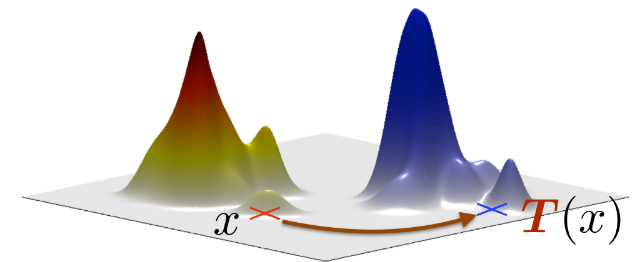
\includegraphics[width=.5\textwidth]{figures/Image2.png}
        \caption{Source : \citep{cuturi_fast_nodate}}
        \label{fig:update}
    \end{figure}
    Le problème de Monge est donc un problème d’optimisation sous contrainte sur un espace fonctionnel, et comme tout problème d’optimisation des questions naturels se posent :
    \begin{itemize}
        \item Existe toujours des solutions ?
        \item Les solutions s’elles existent sont-elles uniques ?
        \item Peut-on caractériser ces solutions ? Et surtout peut on les calculer ?
    \end{itemize}

    Malheursement, dans son mémoire Monge n’a pas pu répondre à ces questions même dans le cas des mesures absolument continues dans l’espace physique et il n'a pu trouver que quelques propriétés géométriques intéressantes de l’application transport optimal s’il existe dont on cite une : "Si le coût est la distance euclidienne alors on ne pourra jamais trouver deux trajectoires qui se coupent". Bien que ces questions soient anciennes il fallait attendre deux siècles pour avoir des réponses satisfaisantes. Notamment en 1941 lorsque \citet{kantorovitch_translocation_1958} (Prix Nobel d’économie) a donné une nouvelle reformulation mathématique du problème du transport optimal plus souple et facile à manipuler en relaxant la contrainte de Monge.

    Pour comprendre pourquoi la théorie n’a pas pu se développer avant Kantorovitch remarquant que le problème de Monge n’admet pas toujours de solution, en effet l’ensemble des contraintes peut être vide (par exemple si $\mu$ est une mesure de Dirac et $\nu$ est une mesure absolument continue ou la moyenne de deux Dirac distincts). En général l’ensemble des contraintes de Monge n’est pas convexe et même s’il est non vide on n’aura pas toujours l’unicité (voir la figure \ref{fig:figure}).
    \begin{figure}[H]
        \centering
        % \hspace*{-9pt}
        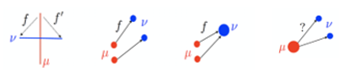
\includegraphics[width=.5\textwidth]{figures/Image3.png}
        \caption{Source : \citep{flamary_optimal_nodate}}
        \label{fig:figure}
    \end{figure}
    \subsection{Formulation de Kantorovich (1942)}\label{sec:kantorovich}
    Dans son étude au problème d’allocation des ressources, Kantorovitch a été amené à étudier un problème de transport optimal entre deux mesures discrètes. Mais dans ce cas, lors du transport des ressources un agent économique peut transférer sa richesse sur plus qu’un agent cible. Et c’est là où réside la différence fondamentale entre la formulation de Kantorovitch et celle de Monge. Dans la formulation de Kantorovitch on peut diviser la masse d’un point $x$ de la distribution de départ de tel sorte qu’une partie de cette masse sera transporté à plusieurs points de la distribution cible.
    Par conséquent, on peut transporter la mesure $\mu$ vers $\nu$ de l’exemple \ref{fig:update} alors que ce n’était pas possible dans le cas de Monge.
    \begin{figure}[H]
        \centering
        % \hspace*{-9pt}
        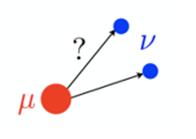
\includegraphics{figures/Image1.png}
        \caption{Source : \citep{flamary_optimal_nodate}}
        \label{fig:update}
    \end{figure}
    Remarquons que dans ce nouveaux point de vue, le transport entre deux mesures ne pourra pas être décrit par une application de transport (car la masse présente en $x$ peut se repartir dans plusieurs positions de l’espace). Mais plutôt par une notion plus générale celle du Couplage entre deux mesures.

    \subsubsection{Noyaux et couplages.}
    L’idée de permettre de casser la masse dans un point $x$ peut être formalisé en associant à chaque point $x$ de la distribution de départ une distribution de probabilité $p_x$ qui modélise la distribution de masse transportée de $x$ dans l’espace $Y$. l’application $p$ qui associe à chaque $x \mapsto p_x$ est appelé un noyau sur $X$.

    Etant donné une mesure source $\mu$ et un noyau $p$, alors on peut transporter $\mu$ par $p$ en une mesure $\nu$ de tel sorte que :
    \[
        \text{Pour tout borélien } \mathcal{B}; \nu(\mathcal{B}) = \int p_x(\mathcal{B}) \,d\mu(x)
    \]
    Qu'on la note par : $\nu = p \star \mu$.

    La masse transportée vers $\mathcal{B}$ depuis $\mu$ est la somme des masses transportées vers $\mathcal{B}$ depuis chaque point $x$ de l’espace.

    Notons que pour que $\nu$ soit définie, la définition précédente de noyau n’est pas suffisante. Pour cette raison on exige de plus que pour toute fonction $f$ mesurable bornée que la fonction : $x \mapsto \int f(y) p_x(\,dy)$ est mesurable.

    Enfin, la formulation de Kantorovitch consiste à remplacer la notion de transport de mesure  dans celle de Monge par le noyau de transition $p$ :
    \[
        \inf_{\nu = p \star \mu} \int_{\mathbb{\Omega \times \Omega}} c(x,y) \,dp_x(y) \,d\mu(x)
    \]
    Or, cette formulation n'est pas souvent présentée dans la littérature et elle n'est qu'une voie équivalente et instructive à la formulation classique et historique de Kantorovich.
    La formulation de Kantorovitch est la suivante :

    \begin{align*}
        \text{\large{(K) : \qquad}} &
            \inf_{\pi \in \Pi(\mu,\nu)} \int_{\mathbb{\Omega \times \Omega}} c(x,y) \,d\pi(x,y) \\
    \end{align*}
    Avec $\Pi(\mu,\nu)$ désigne l’ensemble des mesure de probabilités sur $\Omega \times \Omega$ tel que sa première marginale est $\mu$ et sa deuxième marginale est $\nu$.

    Pour illustrer cette notion de couplage : remarquons que dans la figure \ref{fig:figureh} un couplage entre $\mu$ et $\nu$ est une densité sur l’espace produit représenté en orange. \\
    Déplacer $\mu$ à $\nu$ par ce couplage consiste à dépasser la masse de $\mu$ selon l’axe $y$ de tel façon qu’on reconstruit la répartition orange. Ensuite déplacer la masse orange selon l’axe $x$ de tel façon qu’on reconstruit $\nu$.

    \begin{figure}[H]
        \centering
        % \hspace*{-9pt}
        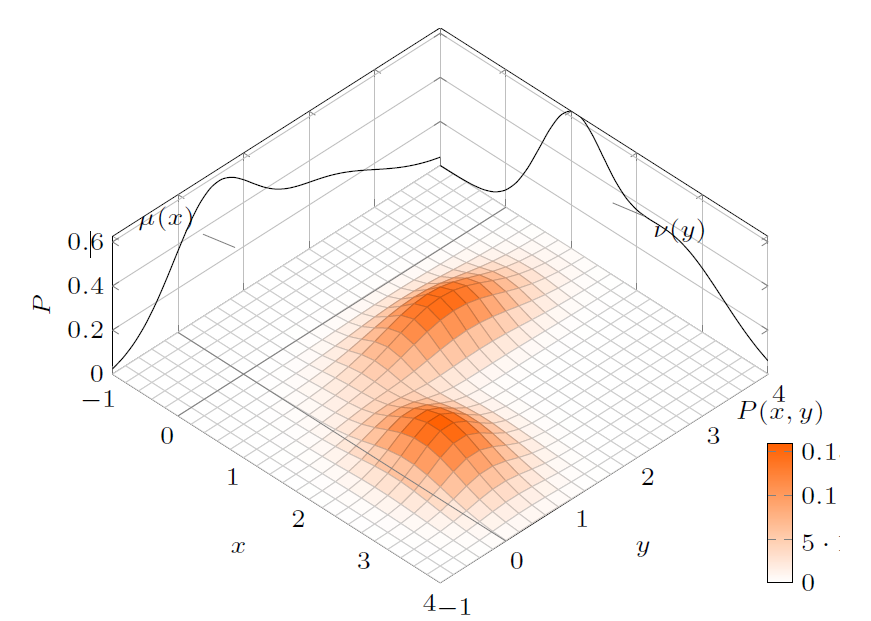
\includegraphics[width=.5\textwidth]{figures/Image4.png}
        \caption{Source : \citep{cuturi_fast_nodate}}
        \label{fig:figureh}
    \end{figure}

    Pour voir le lien entre la formulation par noyaux et la formulation par couplages il est utile de voir $\mu$ et $\nu$ comme la loi de deux variables aléatoires.

    Si $X$ une variable aléatoire qui suit la loi $\mu$ et $Y$ une variable aléatoire qui suit $p_x$ conditionnellement à $X=x$, alors $Y$ suit la loi $v=p \star \mu$. Ainsi le couple $(X, Y)$ suit la loi $\pi$ donné par : $\pi (A \times B)= \int_{A} p_x(B) \,d\mu(x)$. De plus $\pi$ est un couplage entre $\mu$ et $\nu=p \star \mu$. \\
    Autrement dit à partir d’un noyau et une mesure source $\mu$ on peut obtenir un couplage entre $\mu$ et $\nu= p \star \mu$.

    Réciproquement, à partir d’un couplage $\pi$ entre $\mu$ et $\nu$ on peut trouver un noyau de tel sorte que $v= p \star \mu$ et $\pi (A\times B)= \int_{A} p_x(B) \,d\mu(x)$. \\
    De plus ce noyau est unique $u-$presque partout (c’est exactement la conditionnelle de $Y$ sachant $X$ avec $(X, Y)$ est un couple de variable aléatoire distribuer selon $\pi$). \\
    Ainsi dans le cas où $\mu$ et $\nu$ sont soit à la fois discrètes ou continues on peut expliciter la loi de ce noyau en fonction des lois de $\mu$ et $\nu$ \citep{Notes}.

    Finissons cette partie en citant deux couplages particuliers :
    \paragraph{Le couplage indépendant}
    Correspond à la loi jointe de $X$ et $Y$ indépendantes distribué selon $\mu$ et $\nu$ respectivement. En termes de noyau on a : $p_x=\nu$ pour tout $x$ (tous les éléments de masse se repartissent selon $\nu$ indépendamment de l’endroit d’où ils partent).

    \paragraph{Le couplage déterministe.} C’est le cas où il existe une application $T$ de transport de $\mu$ vers $\nu$ tel que le couplage est la loi du couple $(X, T(X))$ avec $X$ suit la loi $\mu$. En termes de noyau on a : $p_x=\delta_{T(x)}$.


    \subsubsection{Avantages théoriques.} Contrairement au problème de Monge, le problème de Kantorovitch est bien posé. Cela est dû au fait que l'ensemble des contraintes est non vide (couplage indépendant). Ainsi, le problème de Kantorovitch est symétrique par rapport à $\mu$ et $\nu$.\\
    De plus le problème de Kantorovitch est un problème d'optimisation linéaire en dimension infinie (dimension finie si les deux mesures sont discrètes) et donc on peut appliquer les méthodes de la théorie du calcul des variations  à ce problème et en particulier à l'existence d'un minimum en montrant sous une condition de continuité où semi-continuité sur le coût et avec un argument de compacité qu'une séquence minimisante de Kantorovitch converge vers un plan optimal ( Avec une notion propre de convergence dans l'espace des mesures de probabilité) \citep{Notes}.
    \begin{theorem}[Existence des plans optimaux]
            Soit $c : \Omega \times \Omega \rightarrow \mathbb{R}^+$ une fonction de coût semi-continue inférieurement. Si $\Omega$ est un espace polonais (séparable et complet); Alors, il existe un plan de transport optimal entre $\mu$ et $\nu$. \citep{santambrogio_optimal_2015}
    \end{theorem}

    Compte tenu de ce qui précède, le problème Kantorovitch est plus facile à traiter du point de vue théorique. Cela vient du fait que Kantorovitch a trop relaxé le problème de Monge. Notez également que Kantorovitch n'est pas une version plus générale que Monge (résoudre Kantorovitch (K) n'implique pas résoudre Monge (M)). Nous pouvons remarquer que la valeur minimale de Kantorovitch est toujours inférieure où égale à celle de Monge (avec la convention $\inf (M) = +\infty$ si l'ensemble des contraintes est vide). \\
    Par ailleurs, nous pouvons montrer que si un plan optimal de (K) est déterministe associé au transport optimal $T$ alors $\inf (M) = \inf (K)$ et $T$ est aussi un transport optimal de (M) (la réciproque reste vraie). \\
    Par conséquent, la résolution du problème de Monge revient à résoudre le problème de Kantorovitch et à voir si sa solution est déterministe \citep{santambrogio_optimal_2015}.

    En complément de toutes ces considérations, qui montrent l'avantage de la formulation de Kantorovitch, nous pouvons introduire un problème dual de Kantorovitch, que l'on note (D). Cette dualité est sans saut ( c'est-à-dire $\inf (K) = \sup (D)$ ) pour des hypothèses particulières sur le coût, ce qui a permis de caractériser des plans optimaux.

    \subsection{Problème dual}\label{sec:dual}
    Une des grandes conséquences de la formulation de Kantorovitch est qu’on peut lui associer un problème dual ($D$).
    Or, notre problème est d'optimisation sous contraintes convexes. La forme dual s'écrit comme suit :
    \begin{definition}[Dualité de Kantorovich]\label{th:dual-k}
        Soit la fonction coût $c : \Omega \times \Omega \rightarrow \mathbb{R}^+$, $\mu$ et $\nu$ deux densités de probabilités. La forme dual ($D$) est :
        \begin{align*}
            \text{\large{(D) : \qquad}} &
            \sup_{\phi(x) + \psi(y) \leq c(x+y)} \int \phi \,d\mu + \int \psi \,d\nu \\
        \end{align*}
        Où $(\phi,\psi) \in L_1(\mu) \times L_1(\nu)$.
    \end{definition}

    \begin{definition}
        Soit $\chi : \Omega \rightarrow \overline{\mathbb{R}}$ une fonction, on définie la $c-$transformé concave de $\chi$ par :
        \[
            \chi^c(y) = \inf_{x \in \Omega} c(x,y) - \chi(x)
        \]
    \end{definition}

    La formulation dual est intéressante car il est plus simple de manipuler des fonctions que manipuler des couplages et surtout d’un point de vue numérique où il est plus facile de stocker des fonctions dans la mémoire qu’à stocker des couplages.

    Des questions naturelles se posent maintenant : Est-ce que le problème admet des solutions ? Est ce qu’on peut les caractériser ? Et si oui, quelle relation avec les solutions optimales de ($D$) et le transport optimal de ($K$) ?

    Commençons par l’existence, la première difficulté de cette formulation dual est que l'ensemble des contraintes n'est pas compact et que nous ne pouvons donc pas obtenir facilement un résultat d'existence comme nous l'avons vu avec ($K$). \\
    Pour surmonter cette difficulté, nous pouvons réécrire ($D$) sous une autre forme avec un ensemble de contraintes compact et une seule fonction $c-$concave au lieu de deux
    \begin{equation} \label{eq:formulation}
        \sup(D) = \sup_{\psi \in \Psi_c(\Omega)} \int_{\Omega} \psi \,d\mu + \int_{\Omega} \psi^c \,d\nu
    \end{equation}
    Où $\Psi_c(\Omega)$ est l'ensemble des fonctions $c-$concaves.

    Ainsi cette égalité a lieu (c’est-à-dire une égalité de dualité et de l’existence d’une solution optimale de $D$ qu’on l’appelle un potentiel de Kantorovitch) si $\Omega$ est polonais et $c$ uniformément continue. \citep{Notes}\\
    Une autre condition suffisante pour satisfaire ce résultat est $\Omega$ compact et $c$ continue. \citep{santambrogio_introduction_2010}

    Notons que dans le cas très général $\inf (K)$ est inférieur à $\sup (D)$ et la différence entre ces deux quantités s’appelle le saut de dualité entre ($K$) et ($D$).

    La nouvelle formulation ci-dessus avec des fonctions $c-$concave montre que la valeur du transport optimal $\inf K$ est convexe par rapport à $\mu$ et $\nu$.

    \subsubsection{Potentiels de Kantorovitch.}
    \begin{definition}
        L'ensemble des fonctions $\psi$ maximisant le problème \ref{eq:formulation} sont appelées les potentiels de Kantorovitch pour le transport de $\mu$ à $\nu$.
    \end{definition}
    Maintenant, nous souhaitons caractériser les potentiels de Kantorovich pour résoudre le problème primal. Cependant, c'est très difficile car nous ne savons pas comment le faire avec des coûts généraux. Mais nous pouvons trouver des résultats remarquables si nous nous intéressons à un coût proportionnel à une puissance de la distance (ce qui n'est déjà pas mal car de tels coûts couvrent la majorité des situations pratiques où l'on s'intéresse aux problèmes de transport). \\
    Dans ce cas on peut montrer \citep{santambrogio_optimal_2015} que sur un compact bornée les fonctions $c-$concaves sont : $pD^{p-1}-$lipschitzienne, avec $p$ la puissance de la distance dans le coût et $D$ le diamètre d’un tel domaine. De plus, lorsque $p=1$ et $p=2$, la fonction de coût est $c = \left( d(x,y)^p /p\right)$. On obtient les caractérisations suivantes :
    \begin{equation*}
        \psi \in \Psi_{1}{(\Omega)} \Longleftrightarrow \psi \text{ est } 1- \text{lipschitziennes}
    \end{equation*}
    \begin{equation} \label{eq:1}
        \psi \in \Psi_{2    }{(\Omega)} \Longrightarrow x\mapsto \frac{x^2}{2}-\psi(x) \text{ est convexe}
    \end{equation}

    On suppose que $\Omega$ est un ouvert compact de $\mathbb{R}^d$.
    \begin{theorem}[Cas d'un coût de la forme $h(x-y)$ où $h$ est strictement convexe]\label{th:cout-s-convexe}
        Si la mesure $\mu$ est à densité par rapport à la mesure de Lebesgue et la frontière de $\Omega$ est $\mu-$négligeable, et il existe au moins un plan optimal qui couple $\mu$ et $\nu$, alors :
        \begin{itemize}
            \item Le plan optimal qui couple $\mu$ et $\nu$ est unique, et il est déterministe (On note $T$ l’application transport associé à ce plan).
            \item Il existe un potentiel $\psi$ de Kantorovitch dont le gradient est unique $\mu-$presque partout.
            \item $T$ et $\psi$ sont relier par la formule suivante $\mu-$presque partout :
            \begin{equation}\label{eq:eqya}
                T(x) = x - \left( \nabla{h^*} \right) \left( \nabla{\psi(x)} \right)
            \end{equation}
        \end{itemize}
    \end{theorem}
    Réciproquement, si une application peut s’écrire de la forme \ref{eq:eqya} $\mu-$presque partout avec $\psi$ une fonction $c$ concave, alors cette application est un transport optimal du problème du Monge \citep{santambrogio_optimal_2015, Notes}.
    \paragraph{Remarques. \citep{santambrogio_optimal_2015, Notes}}
    \hfill \break
    \begin{itemize}
        \item Si $\mu$ est positive. Alors, on peut prouver que le potentiel $\psi$ est unique à une constante additive près.
        \item Si $\mu$ est à densité et $T$ une application vérifiant \ref{eq:eqya} $\mu$-presque partout avec $\psi$ une fonction $c-$concave. Alors, $T$ est un transport optimal entre $\mu$ et l’image de $\mu$ par $T$.
        \item Le résultat reste vrai si on suppose que $\nu$ est à densité au lieu de $\mu$ à condition de remplacer $\mu-$presque partout par $\nu-$presque partout.
        \item Si $\Omega$ est compact l’hypothèse d’existence d’un plan optimal sera automatiquement satisfaite.
    \end{itemize}

    En particulier, pour un coût de la forme $c(x,y) = h(x-y) = \left( d(x,y)^p / p \right)$ avec $p > 1$  la théorème \ref{th:cout-s-convexe} peut caractériser le transport optimal de Monge.

    En utilisant la caractérisation des fonctions $c-$concaves, dans le cas où $p=2$ et $\Omega = \mathbb{R}^d$. Alors, la caractérisation de $T$ devient plus simple et $T = \nabla{\psi}$ où $\psi$ est convexe (c'est le théorème de Brenier \citep{Notes}). \\
    Pour $p = 1$, le coût $c$ ne peut pas être de la forme $h(x-y)$ avec $h$ est strictement convexe, et donc, on ne peut pas appliquer la théorème \ref{th:cout-s-convexe}. Cependant, un théorème similaire peut être obtenu en ce qui concerne l'unicité du plan de transport optimal et son caractère déterministe, mais la caractérisation du transport optimal est plus compliquée et, en pratique, peu utile.

    Deux formulations plus simples pour ce cas peuvent donc être obtenues en utilisant \ref{eq:1}.
    \begin{proposition}
   L'équation \ref{eq:formulation} peut être reformulé comme :
        \begin{small}
            \begin{align*}
                \inf{K} &=& \max_{\psi   \text{ $1-$lipschitzienne}} \int \psi \,d(\mu-\nu) \\
                        &=& \text{Le minimum du problème du flou infimale}\\
                        && \text{de Beckmann \citep{santambrogio_introduction_2010}}
            \end{align*}
        \end{small}
    \end{proposition}
    \paragraph{Quelques considération théorique. \citep{santambrogio_optimal_2015, Notes}} Finissons cette partie par quelques considération théorique :
    \begin{enumerate}[i]
        \item Le théorème \ref{th:cout-s-convexe} reste vrai dans un ouvert de $\mathbb{R}^d$ non compact à condition que $\nu$ soit à support compact et que de plus $\mu$ est à densité dont la frontière de l’intérieur de son support est négligeable et que la valeur $\inf (K)$ est finie.
        \item On peut remplacer la condition de \textit{$\mu$ est à densité} par n’importe quelle condition générale qui assure que l’ensemble des points ou un potentiel de Kantorovitch est non différentiable est négligeable.
        \item Notons qu’on aura encore l’unicité du plan optimal dans le théorème \ref{th:cout-s-convexe} sans que la frontière de $X$ soit négligeable (cependant il ne sera pas forcément déterministe).
        \item Pour le cas d’un coût proportionnele à la puissance d’une distance (non euclidienne), le théorème \ref{th:cout-s-convexe} reste vrai en supposant seulement que $\inf (K)$ est finie.
        \item Un autre cas où le théorème de Bernier reste vrai est celui où deux variables aléatoires de lois respectives $\mu$ et $\nu$ admettent un moment d’ordre 2 et que $\mu$ est sans masse sur tout surface de dimension $d-1$ de classe $\mathcal{C}^2$.
        \item On peut obtenir une version plus générale du théorème \ref{th:cout-s-convexe} avec des coûts plus généraux réguliers. Mais pour une introduction à la théorie du transport optimal et leurs applications le théorème \ref{th:cout-s-convexe} est largement suffisante.
    \end{enumerate}

    \subsection{Quelques cas intéressants}\label{sec:deuxcas}
      Dans son cadre le plus générale, le problème du transport optimal n’est pas facile à résoudre. Cependant, il existe deux cas très particuliers ou on sait trouver d’une manière explicite ou calculer directement le transport optimal : c’est le cas de la dimension 1 et le cas du transport entre deux mesures discrètes.En effet, ces deux cas sont très intéressants en pratiques et permettent d'englober une panoplie d’application très diversifié.


    \subsubsection{Le problème du transport optimal discrèt}
    Dans le cas de deux mesures discrètes $\mu = \sum_{1 \leq i \leq m} p_i \delta_{x_i}$ et $\nu = \sum_{1 \leq j \leq n} q_j \delta_{y_j}$ dans le problème (K), un couplage $\Pi$ sera de la forme :
    \begin{align*}\label{eq:P}
        &\Pi = \sum_{i,j} \Pi_{ij} \delta_{\{x_i\} \times \{y_j\}} &
        \text{avec} & \begin{cases}
            \sum_{j} \Pi_{ij} = p_i \\
            \sum_{i} \Pi_{ij} = q_j \\
            \Pi_{ij} \geq 0
        \end{cases} &
    \end{align*}
    Ainsi, le coût du transport sera entièrement déterminé par la matrice $C = \left( c_{ij} = c(x_i,y_j) \right)$. D'où, le problème (K) sera dans ce cas un problème d'optimisation linéaire en dimension finie :
    \begin{align*}
        \text{\large{(P) : \qquad}} & \begin{cases}
            \inf_{} \langle c,\Pi \rangle = \sum_{i,j} c_{ij} \Pi_{ij}\\
            \Pi \in \mathbb{R}^{m \times n} \\
            \Pi \cdot \mathbb{1}_m = p \\
            \Pi \cdot \mathbb{1}_n = q \\
            \Pi \geq 0 \\
        \end{cases}
    \end{align*}

    et son problème dual associé s'écrit :
    \begin{align*}
        \text{\large{(D) : \qquad}} & \begin{cases}
            \inf_{} \langle p, u \rangle + \langle q, v \rangle\\
            u \in \mathbb{R}^m \\
            v \in \mathbb{R}^n \\
            u_i + v_j \leq c_{ij}
        \end{cases}
    \end{align*}

    Vue que l'ensemble des contraintes est non vide, et bornée (couplage indépendant). Le problème (P) admet toujours une solution. plus généralement, la théorie de programmation linéaire nous annonce que :
    \begin{enumerate}[i] \label{refer}
        \item (P) et (D) admettent au moins une solution et $\max D = \min D$.
        \item Si $\Pi$ est solution de (P) et (u,v) solution de (D), alors,
        \[
            \Pi_{ij} > 0 \Rightarrow u_i + v_j = c_{ij}
        \]
        \item Si $(u,v)$ solution de (D), alors :
        \[
            \begin{cases}
                u_i = \min_{j} (v_j - c_{ij}) \\
                v_j = \min_{i} (u_i - c_{ij})
            \end{cases}
        \]
    \end{enumerate}
    Nous verrons à la fin de cet article que ces résultats peuvent servir à quelques applications en économie.

    Dans le cas où $n=m$ et $p_i = q_j = 1/n$, et grâce à un lemme . les solutions du problème (P) sont déterministe et résout le problème du Monge discrèt suivant (qui n'est rien qu'un problème d'assignement).
    \[
        \min_{\sigma \in \delta_n} \sum_{i} c_{i, \sigma(i)}
    \]

    Enfin, le problème du transport optimal discret se ramène soit à un problème d'optimisation linéaire, où sous forme standard d'assignement. De tels problèmes sont beaucoup étudiés dans la littérature et peuvent être résolus par plusieurs algorithmes (simplexe, simplexe révisé, points intérieurs, flot minimal, hongrois, \dots etc).
    \begin{figure}
        \centering
        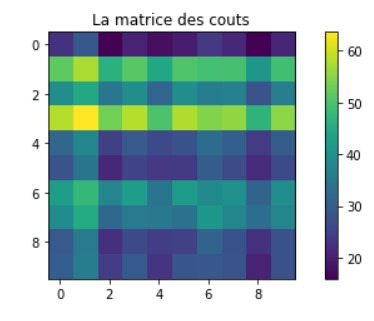
\includegraphics[width=.5\textwidth]{figures/image7.jpg}
        \caption{Le coût du transport optimal}
        \label{fig:my_label}
    \end{figure}
        \begin{figure}
        \centering
        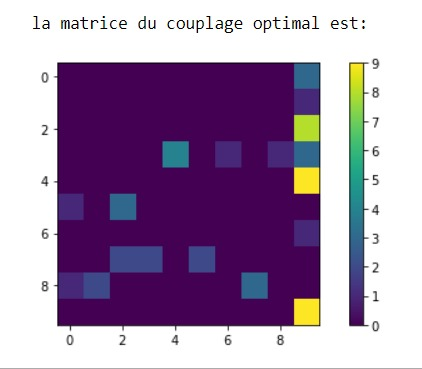
\includegraphics[width=.5\textwidth]{figures/image8.jpg}
        \caption{Le coût du transport optimal}
        \label{fig:my_label}
    \end{figure}
    \begin{figure}[H]
        \centering
        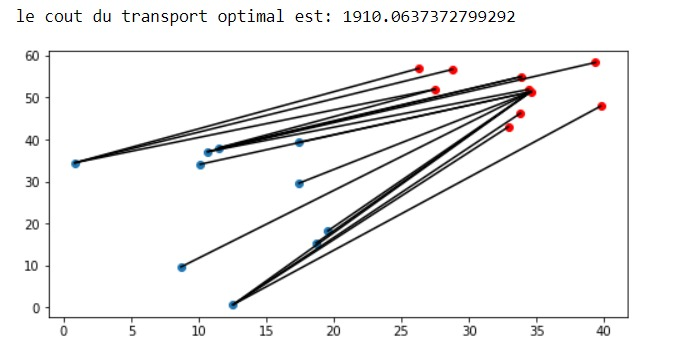
\includegraphics[width=.5\textwidth]{figures/image9.jpg}
        \caption{Simulation du couplage optimal entre deux distributions aléatoires dans le plans. Source : \href{https://github.com/maranibadr/tranport-optimal/blob/master/notebooks/TO_simulation_transport.ipynb}{[Our GitHub]}}
        \label{fig:my_label}
    \end{figure}

    \subsubsection{Le transport optimal sur la droite réelle}
    Dans le cas des mesures définies sur la droite réelle, la notion "d'ordre" nous permet à résoudre le problème du transport optimal d'une manière explicite.
    \begin{theorem}
        Notons par $F^{-1}$ l'inverse généralisé de la fonction de répartition d'une mesure.

        Si le coût est de la forme $h(x-y)$ où $h$ est strictement convexe et $\inf K < \infty$, alors, il existe un unique transport optimal qui est monotone croissant (décroissant si $h$ strictement concave).

        De plus, si $\mu$ est sans atomes alors le plan monotone est déterministe et :
        \begin{align*}
            T &= F_{\mu}^{-1} \circ F_{\nu} \\
            \min{K} &= \int_{0}^{1} h \left( F_{\mu}^{-1}(t) - F_{\nu}^{-1}(t) \right) \,dt
        \end{align*}
    \end{theorem}

    \begin{remarque}
        Si $h$ n'est ni strictement convexe, ni strictement concave. Le résultats d'existence d'un plan monotone optimal reste vrai mais sans unicité en général.

        On peut géneraliser ces résultats pour des coûts qui vérifie des conditions de type :
        \[
            c(x,y') + c(x',y) \leq c(x,y) + c(x',y')
        \]
    \end{remarque}

    Dans le cas discrèt, réssoudre le problème du transport optimal en dimension 1 revient à faire un tri (coût de calcul $\mathcal{O}(N \log{N}$).

    \begin{figure}[H]
        \centering
        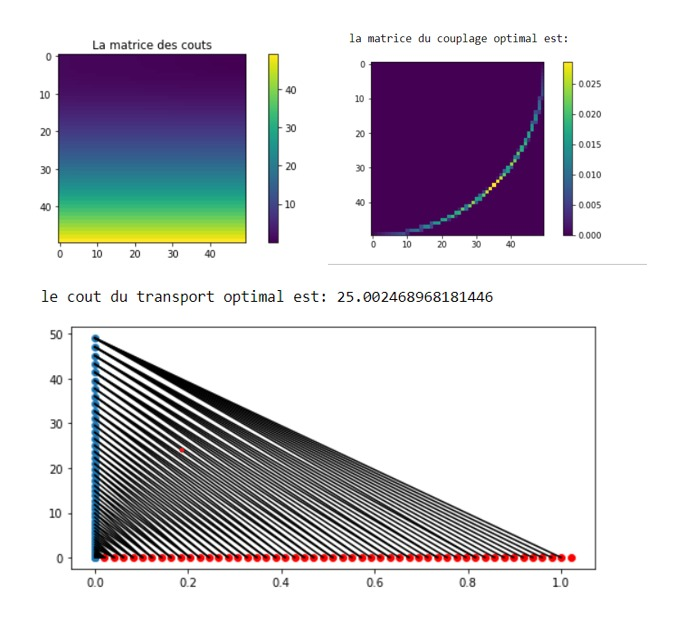
\includegraphics[width=.5\textwidth]{figures/image10.jpg}
        \caption{Simulation d'un transport monotone dans le cas $1D$. Source : \href{https://github.com/maranibadr/tranport-optimal/blob/master/notebooks/TO_simulation_transport.ipynb}{[Our GitHub]}.}
        \label{fig:my_label}
    \end{figure}


    \section{Applications du problème du transport optimal}
    Dans la littérature le transport optimal est utilisé comme un outil pour un large spectre de problème dans plusieurs branches de mathématiques que ça soit pure ou appliqués :  la géométrie, les mathématiques de la physiques, la recherche opérationnelle, l’économie, la finance quantitative, le traitement d’images et des signaux et dans plusieurs problématiques en science des donnés et apprentissage automatique. En effet, la connexion entre la théorie du transport optimal et ces applications polydisciplinaires peut s’expliquer par le fait que le formalisme de cette théorie est lié directement aux notions géométriques et des déformations physiques usuelles qui sont intiment liée au principe du moindre action et à la conservation de masse. Au-delà, le problème du transport optimal permet de définir une distance sur l’espace des mesures de probabilités qui est plus naturel pour comparer et moyenner des distribuions de probabilités tout en gardant la bonne intuition géométrique de ressemblance entre deux distributions dans un espace géométrique, chose qu’on ne le savait pas faire avec des métriques usuels ($L^p$ par exemple).

    Dans cette partie, nous introduisons la distance de Wasserstein en illustrant ses avantages sur des situations pratiques. Nous mettons en évidence les limites de la formulation classique du transport optimal en sciences des données et on présentera le concept de la régularisation entropique à travers le problème de moyennisation des donnés. Enfin, Nous illustrons comment le transport optimal permettra à modèliser des situations d'équilibres et de stabilités en économie.

    \subsection{Distances de Wasserstein}\label{sec:wasserstein}
    Dans le cas où $\Omega$ est un espace metrique compact et pour tout $p \geq 1$, on définit :
    \[
        W_p(\mu,\nu) = \left( \min (K) \text{ avec } c(x,y) = |x-y|^p \right)^{1/p}
    \]
    Où par dualité :
    \[
        \frac{1}{p} W_p^p(\mu,\nu) = \sup_{\psi \in \Psi_p(\Omega)} \int_{\Omega} \psi \,d\nu + \int_{\Omega} \psi^c \,d\mu
    \]

    $W_p$ est une distance sur l'espace $\mathcal{P}(\Omega)$ et la topologie induite par cette distance correspond à la topologie de convergence faible des mesures de probabilités \citep{santambrogio_introduction_2010}.
    \paragraph{Exemple illustratif.} Dans le cas des mesures de probabilités gaussiennes, la distance euclidienne entre deux gaussiennes de même variance est constante dès que leurs supports deviennent disjoints, alors que la distance de Wasserstien est strictement monotone par rapport à la moyenne de la gaussienne cible. Autrement dit, la distance de Wasserstien capture l’intuition du mouvement collective de la masse contrairement aux distances usuels ($L^p$). Nous illustrons ce phénomène avec la simulation suivante :


    \begin{figure}[H]
        \centering
        % \hspace*{-9pt}
        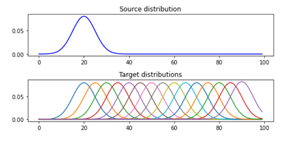
\includegraphics[width=.5\textwidth]{figures/Image5.png}
        \caption{Source : \href{https://github.com/maranibadr/tranport-optimal/blob/master/notebooks/TO_simulation_transport.ipynb}{[Our GitHub]}.}
        \label{fig:figureh}
    \end{figure}

    \begin{figure}[H]
        \centering
        % \hspace*{-9pt}
        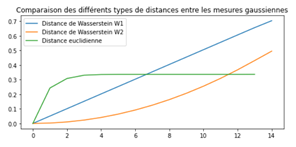
\includegraphics[width=.5\textwidth]{figures/Image6.png}
        \caption{Comparaison des différentes types de distances entre les mesures gaussiennes. Source : \href{https://github.com/maranibadr/tranport-optimal/blob/master/notebooks/TO_simulation_transport.ipynb}{[Our GitHub]}.}
        \label{fig:figureh}
    \end{figure}

    \subsection{Le barycentre de Wasserstein  et moyennisations des donnés empiriques}
    L'agrégation efficace de données provenant de différentes sources est un problème difficile, en particulier lorsque les échantillons de chaque source sont distribués différemment. L'une des façons de fusionner des distributions de probabilités est de le faire par le biais d'un transport optimal.  La méthode du barycentre de Wasserstein \citep{gramfort_fast_2015} est une distribution unique qui résume une collection de mesures d'entrée tout en respectant leur géométrie.


    A travers cette application d’IRM, qui se base sur les idées introduites par Kantorovich \citep{KR:58} afin de proposer un nouvel algorithme capable de calculer efficacement la moyenne de données non normalisées définies sur des domaines discrets arbitraires en utilisant des métriques de transport.

    Elle montre comment les moyennes de Kantorovich peuvent être liées aux barycentres de Wasserstein \citep{agueh_barycenters_2011} afin de tirer parti de l'approche du lissage entropique \citep{cuturi_fast_2014} afin de profiter de l'approche du lissage entropique. Elle conduit à un problème d'optimisation convexe lisse et à un algorithme présentant de fortes garanties de convergence.

    \begin{figure}[H]
        \centering
        % \hspace*{-9pt}
        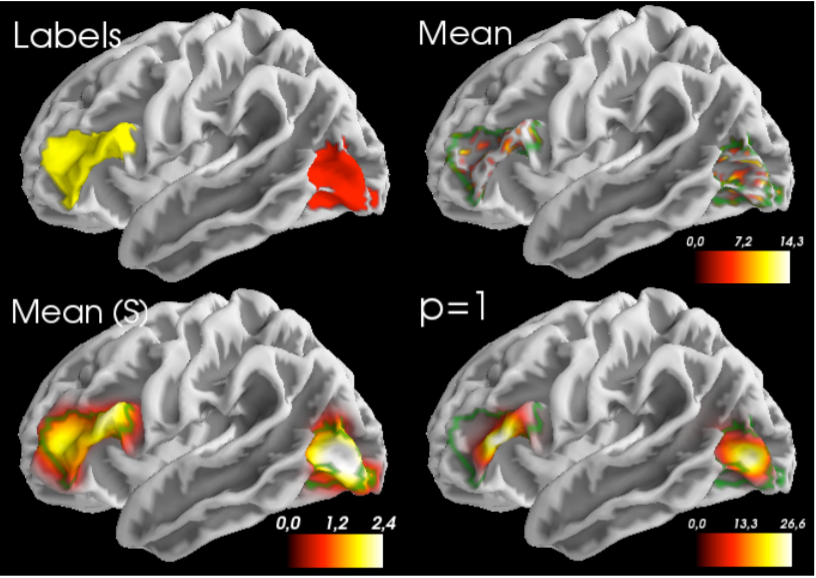
\includegraphics[width=.5\textwidth]{figures/image11.png}
        \caption{Résultats de la simulation avec des signaux aléatoires générés dans un groupe de 100 sujets.}
        \label{fig:figureh}
    \end{figure}

    Cette application illustre la diversité de cet outil et son comportement empirique sur des données de neuroimagerie fonctionnelle, des estimations de sources en IRM fonctionnelle et en magnétoencéphalographie (MEG), définies sur des grilles de voxels et des triangulations de la surface corticale pliée.

    Les données étant volumineuses et d’une grande variabilité, il est difficile de procéder directement à leur lissage. Cependant, en utilisant cette méthode, nous aurons la possibilité de lisser les données que ce soit leurs variabilités et leurs complexités.

    Les contributions de cette méthode sont doubles. Premièrement, en considérant des mesures non-normalisées, particulièrement pertinentes pour les données d'imagerie médicale \citep{thirion_analysis_2007}, nous étendons l'état de l'art actuel dans l'estimation du barycentre en utilisant des métriques de transport.

    Deuxièmement, à la suite de contributions récentes sur le transport optimal discret, cette méthode propose une version lissée du problème de transport qui conduit à un algorithme d’optimisation efficace.  Alors que de nombreuses contributions sur le transport optimal ne travaillent que dans une ou deux dimensions sur une grille régulière, cette approche peut s'adapter à la géométrie complexe du cerveau (grilles et surfaces irrégulières). Seule la définition d'une métrique est nécessaire. L'algorithme proposé implique des opérations simples qui particulièrement adaptées au matériel GPU moderne et qui permet de calculer les barycentres sur des données cérébrales complètes en quelques minutes. Cette méthode a montré la capacité à mettre clairement en évidence les foyers d'activation tout en évitant le besoin de lisser les données.



    \subsection{Application en économie}
    Bien qu’elle a été développé par Kantorovitch lorsqu’il a été confronté à des problèmes économiques, la théorie du transport optimal est presque rarement cité d’une manière explicite dans la littérature économique. C’est seulement dans la dernière décennie que \citet{galichon_optimal_2016} a pu mettre en évidence la connexion directe entre le formalisme du transport optimal et des problèmes économiques fondamentales (les problèmes d’allocations, d’équilibre du marché, d’inversion de demande, et les quantiles multivariés \dots etc.

    En microéconomie, si on suppose que chaque agent économique est rationnel : c’est-à-dire qu’il cherche à maximiser son utilité, on peut caractériser le prix d’équilibre à l’aide d’un problème d’optimisation (Minimisation des surplus des consommateurs et des producteurs, généralement non linéaire) en connaissant les utilités de chaque agent économique.

    Cependant, si on décide de voir les agents économiques comme deux distributions de probabilités discrètes on peut associer à ce marché un couplage qui maximise une utilité globale en connaissant les surplus $\Phi(x,y)$ engendré par la consommation d’un agent $x$ d’une unité de production $y$. Et cette fois ci on affronte un problème linéaire.

    A première vue on pourrait dire que cette modélisation cache la notion d'utilité et de rationalité d'un agent individuel. Nous illustrons à travers l’exemple suivant comment la théorie du transport pourra servir à modéliser ces notions seulement à l'aide d'un problème d'optimisation linéaire, ainsi qu'à  caractériser des prix à l'équilibre.

    \paragraph{Le problème d’affectation et du prix d’équilibre dans un marché.}

    Supposons que nous avons un marché constitué par un ensemble $Y$ de $n$ producteurs d’un bien et d’un ensemble $X$ de $m$ consommateurs prêt à consommer ce bien et notons par $q_y$ la quantité produite par un producteur $y$ et $p_x$ la quantité demandée par un consommateur $x$. On suppose que la demande est égale à l’offre ($ \sum p_x = \sum q_y$). Si on note $\Phi(x,y)$ le surplus engendré entre les agents économiques si $x$ achète une unité du bien du $y$. Le problème d’affectation consiste à trouver les quantités $\Pi(x,y)$ qui représente quantité du bien acheté du bien produit par $y$ de la part des agents $x$ de tel façon que le surplus total sera maximal. Formellement ce problème s’écrit comme un problème du transport optimal, c'est-à-dire :
    \begin{align*}\label{eq:P}
        &\inf_{} \sum_{xy} \pi_{xy} \Phi_{xy} &
        \text{ avec} & \begin{cases}
            \sum_{y} \pi_{xy} = p_x \\
            \sum_{x} \pi_{xy} = q_y \\
        \end{cases} &
    \end{align*}

    Cette notion d’affectation peut être utilisé à plusieurs situations économiques par exemple $X$ des travailleurs et $Y$ des entreprises qui offrent des postions d’emplois pour ces travailleurs.

    Cette fois-ci le problème d’optimisation est linéaire et qui nous permettra de plus définir une notion d’équilibre à travers sa formulation dual. En effet les propriétés i., ii. et iii. en \ref{refer}, nous donne l’intuition d’interpréter les solutions du problème dual associé comme des utilités marginaux associés aux agents économiques du marché qui cherche à les maximiser. En effet, la condition $\mu_i+\nu_j$ supérieur $\Phi(x,y)$ peut s’interpréter par une situation de stabilté car si $\mu_i + \nu_j <  \Phi(x,y)$ alors  les deux agents $x_i$ et $y_j$ ne sont pas en couple d’après ii. en \ref{refer} et ont intérêt à se mettre en couple pour générer un surplus $\mu_i' + \nu_j' = \Phi(x,y)$ plus supérieur à celui qu’avant.

    \paragraph{Hypothèses et notations.}
    \begin{itemize}

        \item Supposons que $\Phi(x,y)=\alpha_{xy} + \beta_{xy}$ avec $\alpha_{xy}$  représente l’utilité de $x$ d’acheter le bien de $y$ et $\beta_{xy}$ représente l’utilité de $y$ de vendre son bien à $x$.

        \item Notons $w_{xy}$ le prix que paye $x$ à $y$ s’il achète une unité de produit.
    \end{itemize}

    \textbf{
    }

    \begin{theorem}[\citep{galichon_optimal_2016}]
        Si on admet que les potentiels de Kantorovitch associé au problème dual du ($P$) représente les utilités des agents et que pour le système des prix $w_{xy}$ à l’équilibre est donné par la maximisation des utilités des agents, c’est-à-dire que :
        \begin{align*}
            \mu_x &= \max_{y} \alpha_{xy} + w_{xy} \\
            \nu_y &= \max_{x} \beta_{xy} - w_{xy}
        \end{align*}

        Alors le système des prix $w_{xy}$ peut être caractérisé par les solutions $(\mu,\nu)$ du problème dual du ($D$).

        Si $\Pi_{xy} > 0$, alors :
        \begin{align*}
            w_{xy} &= \beta_{xy} - \nu_y \\
                   &= \mu_{x} \text{ - } \alpha_{xy}
        \end{align*}
    \end{theorem}

    \section{Conclusion}\label{sec:conclusion}
    Le problème du transport optimal même s’il est ancien n’a cessé d’intéresser les mathématiciens et les scientifiques d’autres disciplines. En effet, cette belle théorie donne un cadre approprié pour capturer des intuitions géométriques complexes et naturelles. Ainsi que sa souplesse en termes d’hypothèses sur les couts et la nature des espaces ou on définit ce transport. Cette souplesse et cette image géométrique que le transport optimal peut capturer dans plusieurs situations complexes ont permis à cette théorie d’être une boite à outils de nombreux problèmes polydisciplinaires, surtout après l’arrivée des méthodes numériques puissantes pour le résoudre d’une manière approchée qui ont donné à cette théorie des nouvelles applications pratiques en sciences des données. Dans ce modeste article, nous avons essayé d’introduire et synthétiser dans des cadres généraux le plus possible les bases théoriques de cette théorie , ainsi qu’à montré par quelques exemples comment cette dernière peut servir à des problèmes déconnectés les uns aux autres à première vue. Finalement, il serait judicieux d’examiner le cas continu et semi-continu afin de pouvoir comprendre le lien entre cette théorie et d'autres domaines telle que la mécanique des fluides et la théorie des jeux.

    \section*{Remerciements}
    Nous tenons à remercier notre encadrant de projet M. Adil Ahidar, enseignant-chercheur en mathématique, pour tout le soutien, le suivi, l’aide, l’orientation et la guidance sans lesquels nous n’aurions pas découvrir et comprendre les bases de cette belle théorie.

\nocite{*}
\begin{footnotesize}
    \bibliography{main.bib}
\end{footnotesize}
\end{document}
